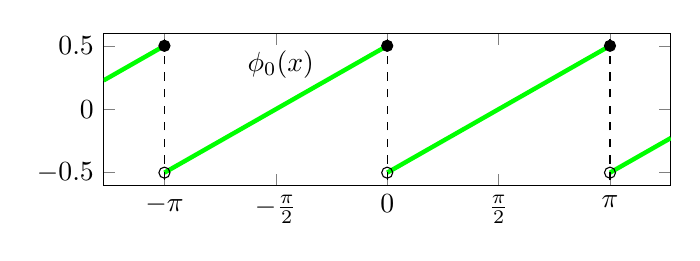
\begin{tikzpicture}
\begin{axis}[
    width=250pt,height=100pt,
    xmin=-4,xmax=4,
    ymin=-0.6,ymax=0.6,
    samples=50,
    xtick={-pi, -pi/2, 0, pi/2, pi},
    xticklabels={$-\pi$, $-\frac{\pi}{2}$, $0$, $\frac{\pi}{2}$, $\pi$},
    grid style={line width=.1pt, draw=gray!10},
    axis line style={latex-latex}]
    
    \addplot[green, ultra thick, domain=-pi:0] (x, x/pi + 1/2);
    \addplot[green, ultra thick, domain=0:pi] (x, x/pi - 1/2);
    \addplot[green, ultra thick, domain=pi:4] (x, x/pi - 3/2);
    \addplot[green, ultra thick, domain=-4:-pi] (x, x/pi + 3/2);

    \addplot[mark=*] coordinates {(-pi,1/2)};
    \addplot[mark=o] coordinates {(-pi,-1/2)};
    \addplot[mark=*] coordinates {(0,1/2)};
    \addplot[mark=o] coordinates {(0,-1/2)};
    \addplot[mark=*] coordinates {(pi,1/2)};
    \addplot[mark=o] coordinates {(pi,-1/2)};

    \draw [dashed] (axis cs:{-pi},-2) -- (axis cs:{-pi},2);
    \draw [dashed] (axis cs:0,-2) -- (axis cs:0,2);
    \draw [dashed] (axis cs:{pi},-2) -- (axis cs:{pi},2);

    \node at (axis cs:-1.5,0.35) {$\phi_0(x)$};
  
\end{axis}
\end{tikzpicture}